\documentclass[conference]{IEEEtran}
\IEEEoverridecommandlockouts
% This TeX installation is missing the PSNFSS Courier outline fonts that
% IEEEtran normally maps \texttt{} to; fall back to Computer Modern
% Typewriter, which ships with every LaTeX installation, to avoid a
% missing-font build failure unrelated to this document's content.
\renewcommand{\ttdefault}{cmtt}

\usepackage{amsmath,amssymb}
\usepackage{graphicx}
\usepackage{booktabs}
\usepackage{algorithm}
\usepackage{algpseudocode}
\usepackage{tikz}
\usetikzlibrary{arrows.meta,positioning}
\usepackage{listings}
\usepackage{xcolor}
\usepackage[hidelinks]{hyperref}

\lstdefinestyle{py}{
  language=Python,
  basicstyle=\ttfamily\scriptsize,
  numbers=left,
  numberstyle=\tiny\color{gray},
  keywordstyle=\bfseries\color{blue!50!black},
  commentstyle=\itshape\color{green!40!black},
  stringstyle=\color{orange!70!black},
  showstringspaces=false,
  breaklines=true,
  frame=single,
  tabsize=4,
  columns=fullflexible,
}

\begin{document}

\title{Decentralized Market-Based Task Allocation for Multi-Robot Teams: From Abstract Simulation to Embodied Webots Validation (Distributed Robotics practical)}

\author{
\IEEEauthorblockN{Halil Elbay, Paul Butter}
}

\maketitle
% TODO before submission: fill in the department name below (assessment
% criteria require "[Surname] is/are with the Department of (TODO),
% Technische Universit\"at Darmstadt, Germany").
\let\thefootnote\relax\footnotetext{H. Elbay and P. Butter are with the Department of (TODO), Technische Universit\"at Darmstadt, Germany.}

\begin{abstract}
Multi-robot teams performing search, surveillance, or logistics tasks must
allocate discovered work among themselves without a single point of
failure. This report studies a decentralized, market-based auction
protocol in which robots bid on tasks from locally computed costs,
benchmarked against nearest-greedy and random-assignment baselines. In an
abstract point-robot simulator, the market strategy achieved a
statistically significant higher operational score, faster completion,
and better load balance across 40 held-out seeds. A subsequent Webots
trial with differential-drive robot models, after correcting several
embodiment-specific calibration issues, reproduced the same qualitative
ranking, supporting the robustness of the decentralized design beyond the
abstract model.
\end{abstract}

\section{Introduction}

Multi-robot task allocation (MRTA) is a recurring requirement wherever a
team of robots must divide discovered work -- inspecting a hazard, guarding
a located object, surveying an area -- without relying on a single
coordinator whose failure would stall the whole team. A centralized
allocator is simple to reason about but forms a single point of failure
and a communication bottleneck that scales poorly with team size; a fully
decentralized scheme trades that fragility for coordination overhead and
a harder-to-predict emergent behavior. Quantifying that trade-off, rather
than merely arguing for decentralization in the abstract, is the concrete
problem addressed in this work.

Market-based coordination for MRTA has a long history, beginning with the
Contract Net Protocol for distributed task announcement and bidding
\cite{smith1980}. Gerkey and Matari\'c provide a formal taxonomy of MRTA
problem classes and note that auction-based methods are a practical
middle ground between fully centralized and fully reactive coordination
\cite{gerkey2004}. Dias~\textit{et al.} survey market-based multi-robot
coordination broadly and highlight that most reported results are
obtained in simulation, with few systematic simulation-to-hardware
comparisons \cite{dias2006}. This report follows that market-based
tradition but adds a specific methodological contribution: the same,
unmodified decentralized decision logic is evaluated first in a fast
abstract simulator and then, without being rewritten, in a
physics-based Webots simulation with embodied differential-drive robots,
so that any gap between the two is attributable to embodiment rather than
to a re-implementation of the strategy.

This report is organized as follows. Section~II formulates the task
allocation problem and the two environments in which it is studied.
Section~III presents the design of the decentralized auction protocol.
Section~IV describes how the design is implemented and how the same
allocation code is reused across both environments. Section~V reports the
holdout results obtained in the abstract simulator and in the Webots
trial. Section~VI discusses the findings, their limitations, and broader
effects.

\section{Problem Formulation}

A team of $N{=}7$ robots operates in a bounded square arena and must
service tasks that appear at scheduled times and locations. Four task
types are defined, each requiring a fixed number of robots to be
simultaneously present, $n_{req}\in\{1,2,3\}$: \texttt{GUARD} (single
robot secures a located object), \texttt{PUSH} (two robots relocate an
object), \texttt{SURROUND} (three robots encircle a spreading hazard),
and \texttt{SURVEY} (single robot re-visits an area whose coverage
information is stale). A task is considered complete once its required
robots have remained within an arrival tolerance of its location for a
fixed duration.

The objective is a weighted operational score
$S=\sum_k w_k\,\hat{m}_k\in[0,1]$ over nine normalized metrics: task
completion rate, mean completion time, region-of-interest (RoI) detection
rate and latency, spatial coverage, workload balance across robots, mean
idleness, avoidance of battery depletion, and remaining battery. Weights
$w_k$ are fixed \emph{before} any parameter search (Table~\ref{tab:score}).

The problem is studied in two environments that share the same task
model and objective but differ in embodiment. In the abstract
environment (Tier~0), robots are dimensionless points that move at a
fixed effective speed with no rotational dynamics; communication has
independent per-link latency and packet loss. In the embodied environment
(Tier~1), robots are Webots e-puck differential-drive models with a
physical radius of approximately $0.037\,\mathrm{m}$, finite rotation and
acceleration, and the same radio abstraction realized as
Emitter/Receiver broadcasts on a shared channel. In both environments,
RoI detection is a disclosed simplification of on-board sensing: a
privileged process (a stand-in for an overhead camera) notifies the
nearest robot once ground-truth distance falls below a detection radius,
matching the fallback sensing model already disclosed in the project
proposal for cases where on-board RoI classification is not available.

\begin{table}[t]
\centering
\caption{Operational score weights, fixed prior to parameter search.}
\label{tab:score}
\begin{tabular}{@{}lr@{\qquad}lr@{}}
\toprule
Component & $w_k$ & Component & $w_k$\\
\midrule
Completion rate & 0.30 & Detection rate & 0.10\\
Completion time & 0.10 & Load balance & 0.15\\
Coverage & 0.05 & Mean idleness & 0.08\\
Detection latency & 0.07 & No depletion & 0.10\\
Remaining battery & 0.05 & & \\
\bottomrule
\end{tabular}
\end{table}

\section{Design}

\subsection{Decentralized auction protocol}

Task assignment uses a peer-to-peer auction with five message types:
\texttt{ANNOUNCE}, \texttt{BID}, \texttt{AWARD}, \texttt{DONE}, and
\texttt{RELEASE}. Any robot that detects a task becomes its
\emph{auctioneer} for that task only; no process ever holds global state
about all tasks or all robots. Algorithm~\ref{alg:auction} summarizes the
lifecycle from the auctioneer's perspective; every other robot runs the
symmetric bidder role concurrently for every task it overhears.

\begin{algorithm}[t]
\caption{Auction lifecycle (auctioneer view)}
\label{alg:auction}
\begin{algorithmic}[1]
\State detect or generate task $\tau$; become auctioneer for $\tau$
\State broadcast \textsc{Announce}$(\tau, n_{req}, \text{deadline})$
\While{now $<$ deadline}
  \State collect \textsc{Bid}$(\tau, \text{cost}, \text{sender})$ from peers
\EndWhile
\State rank bidders by (cost, id); let $W\gets$ cheapest $n_{req}$
\If{$|W| = n_{req}$}
  \State broadcast \textsc{Award}$(\tau, W)$
\Else
  \State retry announcement (bounded attempts) or drop $\tau$
\EndIf
\State \textbf{on} \textsc{Done} \textbf{or} \textsc{Release} from a winner: update local bookkeeping; re-announce if released
\end{algorithmic}
\end{algorithm}

\subsection{Bid cost and priority}

A bidding robot $i$ computes a cost for task $\tau$ from three normalized,
purely local terms -- distance, current workload, and battery deficit:
\begin{equation}
c_i(\tau)=\alpha\,\hat{d}_i+\beta\,\hat{w}_i+\gamma\,(1-\hat{e}_i),
\label{eq:cost}
\end{equation}
with the lowest cost winning. Task priority ages independently of cost,
\begin{equation}
p(\Delta t)=p_0+(1-p_0)\bigl(1-\exp[-(\lambda\Delta t)^k]\bigr),
\label{eq:priority}
\end{equation}
and is used only to arbitrate between a robot's already-assigned task and
a newly announced one. A robot currently navigating toward a task may
preempt it for a higher-priority one if
\begin{equation}
\delta\,(p_{new}-p_{cur})-(c_{new}-c_{cur})>\theta_{hyst},
\label{eq:preempt}
\end{equation}
subject to a cooldown that bounds how often a single robot may switch.
Preemption is disabled once a robot has reached \textsc{Wait\_peers} or
\textsc{Execute}, so a synchronized multi-robot task is never disrupted
after enough winners have arrived.

\subsection{Robot state machine}

Each robot's local control loop is a five-state machine
(Fig.~\ref{fig:fsm}): it \textsc{Explore}s while unassigned,
\textsc{Navigate}s toward its current task once assigned, waits at
\textsc{Wait\_peers} once it has itself arrived but the required team is
incomplete, executes the task once the full team is present, and returns
to \textsc{Explore} on completion. A battery reaching a depletion
threshold moves the robot to an absorbing \textsc{Depleted} state.

\begin{figure}[t]
\centering
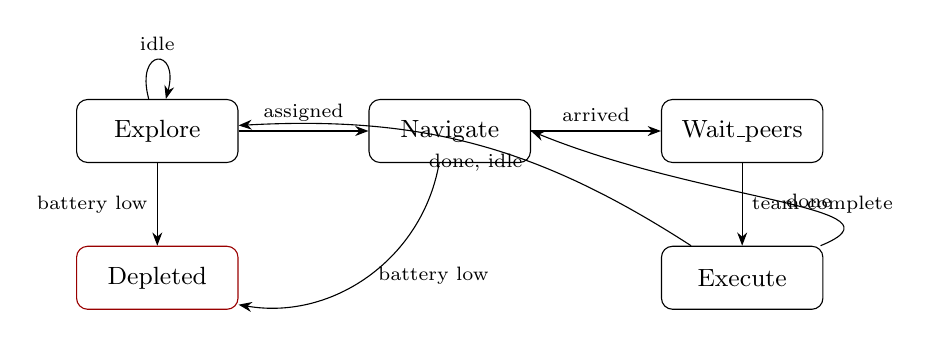
\begin{tikzpicture}[node distance=1.05cm and 1.65cm, >=Stealth,
  state/.style={draw, rounded corners, minimum width=2.05cm, minimum height=0.8cm, align=center, font=\small}]
  \node[state] (explore) {Explore};
  \node[state, right=of explore] (navigate) {Navigate};
  \node[state, right=of navigate] (wait) {Wait\_peers};
  \node[state, below=of wait] (execute) {Execute};
  \node[state, draw=red!60!black, below=of explore] (depleted) {Depleted};

  \draw[->] (explore) -- node[above, font=\scriptsize]{assigned} (navigate);
  \draw[->] (navigate) -- node[above, font=\scriptsize]{arrived} (wait);
  \draw[->] (wait) -- node[right, font=\scriptsize]{team complete} (execute);
  \draw[->] (execute) .. controls +(2.2,0.9) and +(2.2,-0.9) .. node[right, font=\scriptsize]{done} (navigate.east);
  \draw[->] (execute) to[bend right=18] node[below, font=\scriptsize]{done, idle} (explore);
  \draw[->] (explore) to[loop above] node[above, font=\scriptsize]{idle} (explore);
  \draw[->] (explore) -- node[left, font=\scriptsize]{battery low} (depleted);
  \draw[->] (navigate) to[bend left=45] node[right, font=\scriptsize]{battery low} (depleted);
\end{tikzpicture}
\caption{Per-robot finite-state machine. Transitions are driven purely by
locally observable state (own position, own assignments, overheard
messages); no state depends on another robot's internal state.}
\label{fig:fsm}
\end{figure}

\subsection{Embodiment abstraction}

To let Tier~0 and Tier~1 share the identical allocation code, all
platform-specific effects are confined behind an eight-method interface
(read pose, read battery, drive to a point, test arrival, broadcast,
receive, detect RoIs, read time). Tier~0 implements this with point
kinematics; Tier~1 implements it with a non-blocking rotate-then-cruise
controller and Emitter/Receiver radio (Section~IV). The bidding,
priority, and state-machine logic in Sections~III-A to III-C is not
duplicated or modified between tiers.

\section{Implementation}

\subsection{Decision logic}

The allocation package depends only on the Python standard library and is
identical across both tiers. Equation~\eqref{eq:cost} is implemented as
\texttt{compute\_cost} (Appendix~A, lines 24--40); auction ranking and
winner selection follow Algorithm~\ref{alg:auction} directly
(Appendix~B, lines 20--22, a stable sort on (cost, id) tuples that also
guarantees deterministic tie-breaking, which is what makes identical
seeds reproduce byte-identical logs across repeated runs).

\subsection{Tier-0 environment}

The abstract world advances all seven robots with fixed-step point
kinematics, an independent per-link radio model, and a scheduled event
generator that is shared, unmodified, by every strategy under test so
that a given seed produces the same task schedule regardless of which
strategy is being evaluated.

\subsection{Tier-1 Webots environment}

Because Webots ties motor and sensor access to whichever process is
attached as controller of a given robot node, the embodied environment is
$N{+}1$ independent operating-system processes: one per fleet robot, plus
one supervisor process. Each fleet-robot process holds one unmodified
\texttt{allocation} robot instance behind a \texttt{WebotsBackend} that
realizes \texttt{drive\_to()} as a non-blocking rotate-then-cruise state
machine, advanced once per simulation step by \texttt{tick()}
(Appendix~C). A separate supervisor process plays the role of the
overhead camera cited in the project proposal: it reads privileged
ground-truth positions to decide when the required number of winners for
a task have simultaneously arrived (Appendix~D, lines 440--456), and
relays that decision as a broadcast; it never decides \emph{who} wins an
auction, preserving the decentralization of the allocation decision
itself. Both processes also apply a small number of Tier-1-only timing
recalibrations, discussed in Section~VI, implemented as
\texttt{dataclasses.replace()} overrides of the configuration object
rather than as changes to the allocation package.

\section{Results}

\subsection{Tier-0 holdout comparison}

The bid weights (Table~\ref{tab:weights}) were chosen by a grid search over
$\beta,\gamma,\delta,\theta_{hyst}$ restricted to training seeds 0--7. All
reported results use 40 held-out seeds (1000--1039) never used during
parameter selection; every seed is run under all strategies so that a
directed, paired difference can be formed per seed. Table~\ref{tab:tier0}
reports the holdout means; Table~\ref{tab:tier0-effects} reports the
key paired effects, each with a 95\% bootstrap confidence interval (CI,
20{,}000 resamples), win rate, and Holm-corrected $p$-value from a paired
sign-randomization test.

\begin{table}[t]
\centering
\caption{Bid weights selected by the Tier-0 grid search.}
\label{tab:weights}
\begin{tabular}{@{}ccccc@{}}
\toprule
$\alpha$ & $\beta$ & $\gamma$ & $\delta$ & $\theta_{hyst}$\\
\midrule
1.0 & 0.5 & 0.0 & 1.5 & 0.1\\
\bottomrule
\end{tabular}
\end{table}

\begin{table}[t]
\centering
\caption{Tier-0 holdout means over 40 seeds (n=40 per strategy).}
\label{tab:tier0}
\small
\begin{tabular}{@{}lrrrr@{}}
\toprule
Strategy & Score & Completion & Time [s] & Load-SD\\
\midrule
Market & \textbf{0.861} & \textbf{0.918} & \textbf{37.76} & \textbf{1.42}\\
Nearest Greedy & 0.831 & 0.887 & 47.84 & 1.84\\
Random & 0.813 & 0.788 & 59.60 & 1.35\\
\bottomrule
\end{tabular}
\end{table}

\begin{table}[t]
\centering
\caption{Paired Market advantage over baselines, 40 holdout seeds.}
\label{tab:tier0-effects}
\small
\begin{tabular}{@{}lrrl@{}}
\toprule
Comparison & $\Delta$ & 95\% CI & win rate, $p_{Holm}$\\
\midrule
Score vs.\ Greedy & $+0.0305$ & $[0.0151,0.0462]$ & 77.5\%, $0.0040$\\
Time vs.\ Greedy [s] & $-10.08$ & $[-13.72,-6.46]$ & 87.5\%, $<0.05$\\
Score vs.\ Random & $+0.0479$ & -- & significant\\
Time vs.\ Random [s] & $-21.85$ & -- & significant\\
\bottomrule
\end{tabular}
\end{table}

For every reported comparison the confidence interval excludes zero and
$p_{Holm}<0.05$; the market strategy is not merely better on average by
chance across the 40 held-out scenarios. The advantage is not uniform
across every metric: against Nearest Greedy, Market requires on average
about two additional messages per completed task, a difference that
narrowly fails significance after correction, and Random Assignment can
by chance produce a more even load with far fewer tasks completed.

\subsection{Tier-1 Webots trial}

The identical, unmodified allocation code was then run against Webots
e-puck models on one held-out seed (1000), for Market, Nearest Greedy,
and Random Assignment (Table~\ref{tab:tier1}). Unlike the Tier-0 result,
this is a \emph{single run per strategy}, not a statistically powered
holdout comparison, and is reported as such.

\begin{table}[t]
\centering
\caption{Tier-1 Webots trial, single 300\,s run per strategy, seed 1000.}
\label{tab:tier1}
\small
\begin{tabular}{@{}lrrrr@{}}
\toprule
Strategy & Completed & Mean [s] & Median [s] & Load imb.\\
\midrule
Market & \textbf{17} & \textbf{54.6} & \textbf{55.7} & \textbf{1.58}\\
Nearest Greedy & 16 & 72.2 & 76.9 & 1.83\\
Random & 8 & 132.4 & 165.9 & 1.28\\
\bottomrule
\end{tabular}
\end{table}

The ranking Market $>$ Greedy $>$ Random by completion count and speed
matches the Tier-0 ranking. The gap between Random and the other two
strategies is markedly larger than in Tier~0, consistent with a
mechanism discussed in Section~VI: a poorly chosen assignment wastes far
more wall-clock time under real, finite-speed travel than under Tier~0's
abstract kinematics.

Reaching a working Tier-1 trial required diagnosing four
embodiment-specific issues, none of which were present in Tier~0:
(i) an incorrect heading-offset calibration caused robots to orbit their
target at a near-constant radius instead of approaching it, diagnosed
from live trajectories showing a consistent $\approx\!90^{\circ}$ lead of
travel direction over bearing-to-target across three independent robots;
(ii) Tier-0's arrival tolerance ($0.035\,\mathrm{m}$) is smaller than an
e-puck's physical radius, so tasks requiring $n_{req}>1$ robots at one
point could never register all winners as simultaneously arrived, once
real robot bodies physically blocked each other; (iii) the timeout and
preemption-cooldown constants, calibrated for Tier-0's near-instantaneous
motion, caused near-total task starvation at real travel speeds until
rescaled; (iv) an attempt to give \texttt{PUSH} objects real collision
geometry and have winners physically relocate them was implemented and
tested, but the light propped object did not move under Webots' default
contact friction, and the attempt was abandoned in favor of the same
duration-based completion already used by \texttt{GUARD}/\texttt{SURROUND}.

\section{Discussion}

The Tier-0 holdout result is a statistically grounded finding within its
scenario family: at 40 independently sampled seeds, the market strategy's
score, completion-time, and (against Greedy) load-balance advantages are
each significant after multiple-comparison correction. The Tier-1 result
is weaker in kind: a single seed cannot support a confidence interval or
a significance test, and the reported ranking should be read as a
demonstration that the qualitative ordering \emph{can} survive embodied
dynamics, not as proof that it does so reliably. Extending Tier~1 to
multiple held-out Webots seeds, mirroring the Tier-0 protocol exactly,
is the natural next step before the same ranking claim can be made with
comparable confidence.

The four embodiment issues found in Section~V-B are informative beyond
their immediate fixes. Three of the four (heading calibration, arrival
tolerance, timing constants) are properties of a specific simulator and
robot model, not of the allocation strategy, and were resolved without
touching the allocation package -- direct evidence that the chosen
backend abstraction achieved its purpose of isolating decision logic
from embodiment. The fourth (PUSH object relocation) is different in
kind: it is a physical force-closure problem, and its failure under
default contact parameters is consistent with the project proposal's own
prior assessment that push interactions were not expected to be
demonstrable on the real hardware platform. Reporting this failure
rather than omitting it is intentional: a lighter-weight object,
non-default contact friction, or a two-robot squeeze geometry might
succeed, but this was not verified, and claiming otherwise without
evidence would misrepresent the result.

A plausible explanation for the larger Market-Random gap observed in
Tier~1 relative to Tier~0 is that Tier~0's abstract, near-instantaneous
motion makes a poor assignment cheap to recover from, whereas at Webots'
finite travel speed (tens of seconds per traversal) a robot sent to a
distant or already-contested task wastes real time that can no longer be
reallocated within the scenario's duration; this would predict that the
gap should shrink again as travel speed increases relative to task
inter-arrival time, which is a testable hypothesis for future work rather
than a confirmed finding here.

Decentralized task allocation of the kind studied here has a favorable
ecological profile relative to a centralized alternative in one specific
respect: it removes the need for a continuously powered, always-reachable
central compute and communication node, which is a meaningful reliability
and energy consideration for field deployments such as environmental
monitoring or search and rescue, where infrastructure may be unavailable
or unreliable. Set against this, a team of several small robots
generally has a larger combined manufacturing and end-of-life footprint
than one larger robot for the same coverage area, a trade-off that should
be weighed against the resilience gained. The \texttt{GUARD} and
\texttt{SURROUND} task types studied here are structurally close to
autonomous perimeter-control and surveillance behaviors; a real
deployment of this coordination scheme for such purposes would raise
privacy and dual-use considerations that are outside the scope of the
present allocation-efficiency study but should be considered before any
such deployment.

\begin{thebibliography}{9}
\bibitem{smith1980} R.~G. Smith, ``The contract net protocol: High-level
communication and control in a distributed problem solver,'' \emph{IEEE
Trans. Comput.}, vol.~C-29, no.~12, pp.~1104--1113, 1980.
\bibitem{gerkey2004} B.~P. Gerkey and M.~J. Matari\'c, ``A formal analysis
and taxonomy of task allocation in multi-robot systems,'' \emph{Int. J.
Robot. Res.}, vol.~23, no.~9, pp.~939--954, 2004.
\bibitem{dias2006} M.~B. Dias, R.~Zlot, N.~Kalra, and A.~Stentz,
``Market-based multirobot coordination: A survey and analysis,''
\emph{Proc. IEEE}, vol.~94, no.~7, pp.~1257--1270, 2006.
\end{thebibliography}

\onecolumn
\appendix

\subsection*{Appendix A: bid cost (\texttt{allocation/bidding.py})}
\begin{lstlisting}[style=py,firstnumber=24]
def compute_cost(
    robot_pose: tuple[float, float],
    battery: float,
    workload: int,
    task: Task,
    weights: BidWeights,
    d_max: float,
    workload_cap: int = 3,
) -> float:
    """Return bid cost; a lower value is better."""

    if d_max <= 0.0 or workload_cap <= 0:
        raise ValueError("normalisation constants must be positive")
    distance_term = min(dist(robot_pose, task.position) / d_max, 1.0)
    workload_term = min(workload / workload_cap, 1.0)
    battery_term = 1.0 - min(1.0, max(0.0, battery))
    return weights.alpha * distance_term + weights.beta * workload_term + weights.gamma * battery_term
\end{lstlisting}

\subsection*{Appendix B: auction winner selection (\texttt{allocation/auction.py})}
\begin{lstlisting}[style=py,firstnumber=16]
def submit(self, robot_id: str, cost: float, now: float) -> None:
    if now <= self.deadline and cost >= 0.0:
        self.bids[robot_id] = cost

def winners(self) -> list[str]:
    ranked = sorted(self.bids.items(), key=lambda item: (item[1], item[0]))
    return [robot_id for robot_id, _ in ranked[: self.n_req]] if len(ranked) >= self.n_req else []
\end{lstlisting}

\subsection*{Appendix C: Tier-1 non-blocking movement controller (\texttt{backends/webots.py})}
\begin{lstlisting}[style=py,firstnumber=219]
def tick(self, dt: float) -> None:
    """Advance the wheel motors by one Webots time step toward the current target."""

    if self._phase == _Phase.BACKOFF:
        if self.now() < self._backoff_until:
            self.left_motor.setVelocity(BACKOFF_SPEED)
            self.right_motor.setVelocity(BACKOFF_SPEED)
            self._drain_battery(dt, abs(BACKOFF_SPEED) * WHEEL_RADIUS * dt)
            return
        self._phase = _Phase.IDLE

    if self.target is None or self.is_at_target():
        self.left_motor.setVelocity(0.0)
        self.right_motor.setVelocity(0.0)
        self._phase = _Phase.IDLE
        self._drain_battery(dt, 0.0)
        return

    px, py, heading = self.get_pose()
    bearing = math.atan2(self.target[1] - py, self.target[0] - px)

    if self._phase == _Phase.IDLE:
        self._phase = _Phase.ROTATE

    if self._phase == _Phase.ROTATE:
        error = _wrap(bearing - heading)
        if abs(error) <= math.radians(ROTATE_TOLERANCE_DEG):
            self._phase = _Phase.CRUISE
            self._cruise_start = self.now()
            self._stuck_check_pos = (px, py)
            self._stuck_check_time = self.now()
            self.left_motor.setVelocity(0.0)
            self.right_motor.setVelocity(0.0)
        else:
            turn = max(-MAX_WHEEL_SPEED, min(MAX_WHEEL_SPEED, ROTATE_GAIN * error))
            self.left_motor.setVelocity(-turn)
            self.right_motor.setVelocity(turn)
        self._drain_battery(dt, 0.0)
        return

    drift_deg = math.degrees(abs(_wrap(bearing - heading)))
    if drift_deg > REALIGN_THRESHOLD_DEG:
        self._phase = _Phase.ROTATE
        self.left_motor.setVelocity(0.0)
        self.right_motor.setVelocity(0.0)
        self._drain_battery(dt, 0.0)
        return

    if self.now() - self._stuck_check_time >= STUCK_CHECK_INTERVAL_S:
        progress = math.hypot(px - self._stuck_check_pos[0], py - self._stuck_check_pos[1])
        self._stuck_check_pos = (px, py)
        self._stuck_check_time = self.now()
        if progress < STUCK_DISTANCE_THRESHOLD:
            self._phase = _Phase.BACKOFF
            self._backoff_until = self.now() + BACKOFF_DURATION_S
            self.left_motor.setVelocity(BACKOFF_SPEED)
            self.right_motor.setVelocity(BACKOFF_SPEED)
            self._drain_battery(dt, abs(BACKOFF_SPEED) * WHEEL_RADIUS * dt)
            return

    ramp_fraction = min(1.0, (self.now() - self._cruise_start) / CRUISE_RAMP_S)
    speed = CRUISE_SPEED * ramp_fraction
    self.left_motor.setVelocity(speed)
    self.right_motor.setVelocity(speed)
    self._drain_battery(dt, speed * WHEEL_RADIUS * dt)
\end{lstlisting}

\subsection*{Appendix D: privileged $n_{req}$-arrival check (\texttt{docs/webots\_market\_supervisor\_controller.py})}
\begin{lstlisting}[style=py,firstnumber=440]
for task_id, runtime in list(tasks.items()):
    if runtime.winners is None:
        continue
    if runtime.active_at is None:
        if runtime.award_at is not None and now - runtime.award_at > config.assignment_timeout:
            emitter.send(json.dumps({"ctl": CTL_COORD_TIMEOUT, "task_id": task_id}).encode("utf-8"))
            runtime.winners = None
            runtime.award_at = None
            continue
        ready = all(
            pose.get(w) is not None and dist(pose[w], runtime.position) <= config.arrival_tolerance
            for w in runtime.winners
        )
        if ready and len(runtime.winners) == runtime.n_req:
            runtime.active_at = now
            emitter.send(json.dumps({"ctl": CTL_ACTIVE, "task_id": task_id}).encode("utf-8"))
    elif now - runtime.active_at + 1e-9 >= runtime.duration:
        complete_task(task_id, runtime, now)
\end{lstlisting}

\end{document}
